%%===============================================================================
% Document configuration

%%-------------------------------------------------------------------------------
% Document type

%\documentclass[conference]{IEEEtran}
\documentclass[letterpaper, 10pt, conference]{IEEEtran}
%\documentclass[letterpaper, 10pt, conference]{ieeeconf}
% \IEEEoverridecommandlockouts

%%-------------------------------------------------------------------------------
% Package configuration
\usepackage{algorithmic}
\usepackage{amsmath,amsfonts}
\usepackage{booktabs, tabularx}   % allows for \toprule in tables
\usepackage{cite}
\usepackage{graphicx}
\graphicspath{ {./img/} }
\usepackage{multirow}
\usepackage{newtxmath}
\usepackage{ragged2e}
\usepackage{textcomp}
\usepackage{xcolor}

%%-------------------------------------------------------------------------------
% Custom Commands
\newcommand{\TODO}[1]{{\color{green} To do: #1}} % For adding notes to paper

%%-------------------------------------------------------------------------------
% Bibliography
\def\BibTeX{{\rm B\kern-.05em{\sc i\kern-.025em b}\kern-.08em
    T\kern-.1667em\lower.7ex\hbox{E}\kern-.125emX}}

%%-------------------------------------------------------------------------------
% Title
\title{A Position Allocation Approach to Battery Electric Bus Scheduling}

%%-------------------------------------------------------------------------------
% Authors
\author{\IEEEauthorblockN{1\textsuperscript{st} Alexander Brown}
\IEEEauthorblockA{\textit{Department of Electrical and Computer Engineering} \\
\textit{Utah State University}\\
Logan, USA \\
alex.brown7711@aggiemail.usu.edu}
\and
\IEEEauthorblockN{2\textsuperscript{nd} Greg Droge}
\IEEEauthorblockA{\textit{Department of Electrical and Computer Engineering} \\
\textit{Utah State University}\\
Logan, USA \\
greg.droge@usu.edu }}

%%===============================================================================
% Title, Authors, Abstract, Keywords
\begin{document}

%%-------------------------------------------------------------------------------
% Create title
\maketitle

%%-------------------------------------------------------------------------------
% Abstract
\begin{abstract}
[\TODO{Copied}] A major challenge to adopting battery electric buses into bus fleets is the scheduling of the battery charging while considering route timing constraints, battery charge, and battery health. This work develops a scheduling framework to balance the use of slow and fast chargers assuming the bus routes and charger locations are fixed. Slow chargers are utilized when possible for sake of battery health and fast chargers are used when needed to accommodate timing constraints and ensure a sufficient charge for route execution. A directed, acyclic graph is used to model the available charge times for buses that periodically return to a depot for charging. A constrained network flow Mixed-Integer Linear Program (MILP) problem is formulated to optimize the scheduling of chargers as well as to determine the number of chargers required to meet charging thresholds. Results are presented using a randomly generated bus schedule for thirty buses and demonstrate the ability of the planner to consider peak time charging costs while planning with fixed and variable numbers of chargers.
\end{abstract}

%%-------------------------------------------------------------------------------
% Keywords
\begin{IEEEkeywords}

\end{IEEEkeywords}

%%===============================================================================
% Paper

%%-------------------------------------------------------------------------------
% Introduction
\section{Introduction}
\label{sec:introduction}
The public transportation system is crucial in any urban area; however, the increase awareness and concern of environmental impacts of petroleum based public transportation has driven an effort to reduce the pollutant footprint \cite{DeFilippo2014, Xylia2018, Guida2017, Li2016}. Particularly, the electrification of public bus transportation via battery power, known as battery electric buses (BEBs), has received significant attention \cite{Li2016}. Although the technology provides benefits beyond reduction in emissions such as lower driving costs, lower maintenance costs, and reduced vehicle noise; battery powered systems introduce new challenges such as larger upfront costs, and potentially several hour long ``refueling" periods \cite{Xylia2018, Li2016}. Furthermore, the problem is exacerbated by the constraints of the transit schedule the fleet must adhere to, the limited amount of chargers available, as well as the adverse affects in the health of the battery due to fast charging \cite{Lutsey2019}. This paper presents a continuous scheduling framework for a BEB fleet that shares limited fast and slow chargers. This framework takes into consideration linear charging dynamics and a fixed bus schedule while meeting a certain battery percentage threshold while remaining.

[\TODO{Copied}] Recent research seeks to enable BEB fleet deployment by solving two problems: providing BEB scheduling (when to charge, at which charger) and determining BEB infrastructure (charger placement, route design). Much attention has been given to solving both problems simultaneously \cite{Wei2018, Sebastiani2016, Hoke2014, Wang2017}. Additional variations in addressing the infrastructure include determining which existing buses should be replaced by a BEB \cite{Zhou2020}, assignments of buses to routes \cite{Liu2020}, and determining locations of fast wireless chargers along the routes \cite{Yang2018, Wang2017a}. The added complexity of considering both the BEB charge scheduling and the infrastructure problems necessitates simplifications for sake of computation.

[\TODO{Copied}] Two such simplifications are common. First, only fast chargers are utilized in planning \cite{Wei2018, Sebastiani2016, Wang2017, Zhou2020, Liu2020, Yang2018, Wang2017a, Qin2016}. Second, significant simplifications to the charging models are made. Some approaches assume full charge \cite{Wei2018, Wang2017, Zhou2020, Wang2017a}. Others have assumed that the charge received is proportional to the time spent on the charger \cite{Liu2020, Yang2018}, which can be a valid assumption when the battery state-of-charge (SOC) is below 80\% charge \cite{Liu2020}. Day-to-day operations require higher fidelity charging models to ensure buses have sufficient charge and to better incorporate the monetary cost of charging. In \cite{Sebastiani2016, Qin2016}, high-fidelity models are used at the price of requiring computationally intensive searches; \cite{Sebastiani2016} uses a genetic algorithm and \cite{Qin2016} uses an exhaustive search strategy.

The contribution of this work is a Mixed Integer Linear Program (MILP) scheduling framework that considers bus schedules, charging battery dynamics, charge limits, and availability of slow and fast chargers. The bus schedules are assumed to be fixed for the duration of the time horizon. The linear program is formed, and extends upon, the Position Allocation Problem (PAP) \cite{Qarebagh2019}. Linear charging dynamics are assumed, costs are assumed to be constant for the duration of the time horizon, and the amount of chargers is assumed to be constant. The MILD framework allows the addition and replacing of constraints. As such, battery dynamic constraints may be replaced with first-order dynamic modeling and costs can be made dynamic. The solution of the problem provides the arrival time, selected charger (fast or slow), initial charge time, final charge time, and departure time from the station.

The remainder of the paper proceeds as follows.

\begin{table*}[!t]
	\caption{Notation used throughout the paper \TODO{Cleaning up notation a little to make it more sensible}}
	\label{tab:variables}
	\centering
	\begin{tabular}{l l l l}
		\toprule
		\textbf{Variable} & \textbf{Description} & \textbf{Variable} & \textbf{Description} \\
		\toprule
		\multicolumn{4}{l}{Input values} \\
			$T$         & Time Horizon           &
			$N$         & Number of total visits                    \\
			$A$         & Number of buses in use &
			$Q$         & Number of chargers                        \\
			$I$         & Final index            &
			$M$         & An arbitrary very large upper bound value \\
			$\Xi$       & $N(N-1)$                                   \\
		\hline
		\multicolumn{4}{l}{Input Vectors} \\
			$a_i$        & Arrival time of visit  $i$              &
			$m_q$        & Cost of a visit being assigned to charger  $q$                  \\
			$\epsilon_q$ & Cost of using charger $q$ per unit time &
			$r_q$        & Charge rate of charger $q$ per unit time                        \\
			$\Gamma_i$   & Array of visit id's                     &
			$\gamma_i$   & Array of values indicating the next index visit $i$ will arrive \\
			$\tau_i$     & Time visit $i$ must leave the station   &
			$\lambda_i$  & Discharge of visit over route  $i$                              \\
			$\alpha_i$   & Initial charge time for visit  $i$      &
			$\beta_{i}$  & Final charge for bus $i$ at the end of the work day             \\
			$\kappa_i$   & Final charge time for visit $i$                                 \\
		\hline
		\multicolumn{4}{l}{Decision Variables} \\
			$u_i$         & Initial charge time of visit $i$                          \\
			$v_i$         & Assigned queue for visit $i$                  &
			$c_i$         & detach time from charger for visit $i$                    \\
			$p_i$         & Amount of time spent on charger for visit $i$ &
			$g_i$         & Linearization term for bilinear terms $g_i := p_i w_{iq}$ \\
			$\eta_i$      & Initial charge for visit $i$                  &
			$w_{iq}$      & Vector representation of queue assignment                 \\
			$\sigma_{ij}$ & $u_i < u_j = 1$ \textrm{ or } $i \neq j = 0$  &
			$\delta_{ij}$ & $v_i < v_j = 1$ \textrm{ or } $i \neq j = 0$              \\
			\bottomrule
	\end{tabular}
\end{table*}

%%-------------------------------------------------------------------------------
% Preliminaries
\section{Preliminaries}
\label{sec:preliminaries}
The PAP is a rectangle packing problem where a set of rectangles \(\vmathbb{R}\) are attempted to be optimally placed in a larger rectangle \(R\) as shown in Fig \ref{fig:packexample}. Both the set \(\vmathbb{R}\) and rectangle \(R\)'s width and height are used to represent quantifiable values. The rectangle packing problem is a subset of the packing problem and can be used to describe many real life problems \cite{Bruin2013}. One of these problems is the Berth Allocation Problem (BAP).

The BAP is a form of the rectangle packing problem where the set of rectangles describe incoming vessels to a be docked on a berth to be serviced as shown in Fig \ref{fig:bap} \cite{Dai2008}. The BAP is commonly formed as a Mixed Integer Linear Program (MILP) \cite{Frojan2015,Buhrkal2010}. This formulation utilizes the BAP to help determine which queue the bus should be placed on to be charged without violating time or space constraints. Notation is summarized in Table \ref{tab:variables}.

\begin{figure}
	\centerline{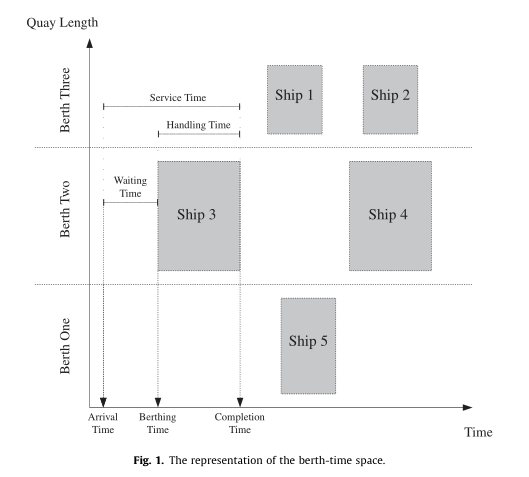
\includegraphics[width=8cm]{bap.png}}
	\caption{The representation of the berth-time space \TODO{Update Image}}
	\label{fig:bap}
\end{figure}

\subsection{The Rectangle Packing Problem}
Rectangle packing can be shown to be a NP-hard problem \cite{Murata1995}. As shown in Fig \ref{fig:packexample}, there is static sized rectangle \(R\) for the set of small rectangles \(\vmathbb{R}\) to be packed into where the width and height are used to represent measurable values provided by the problem. In some problems, the dimensions of \(\vmathbb{R}\) are held constant such as in the problem of packing modules on a chip, where the widths and height of the rectangles represent the physical width and heights of the modules \cite{Murata1995}. Other problems, such as the BAP, allow one or both sides to be decision variables (i.e. the dimension is variable) \cite{Buhrkal2010}.

\begin{figure}
	\centerline{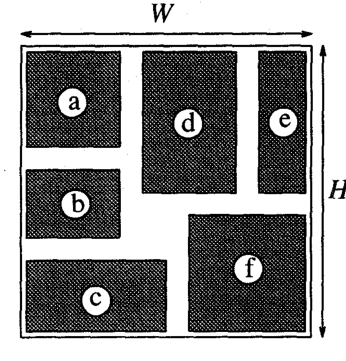
\includegraphics[width=6cm]{chip-pack.png}}
	\caption{Example of rectangle packing problem \TODO{Update Image}}
	\label{fig:packexample}
\end{figure}

\subsection{The Berth Allocation Problem}
The BAP is used to optimally assign incoming vessels to berth positions in order to be serviced (Fig \ref{fig:bap}). The width and height of \(R\) represent the berth length \(S\) and time horizon \(T\), respectively. Similarly, the width and height for \(\vmathbb{R}\) represent the time spent to service vessel $N$ and the space taken by docking vessel $N$, respectively. The vessel characteristics (length of the vessel, arrival time, handling time, desired departure time) are assumed to be known for all $N$ vessels being served.

The BAP has characteristics that are both convenient and undesirable; to explore these, consider the following MILP:

\begin{equation}
	\label{eq:bapobjective}
	min\; \sum_{i=1}^N (c_i - a_i)
\end{equation}

Subject to the following constraints:

\begin{subequations}
\label{eq:bapconstrs}
\begin{align}
    u_i - u_j - p_j - (\sigma_{ij} - 1)T \geq 1                     \label{subeq:baptime}         \\
    v_i - v_j - s_j - (\delta_{ij} - 1)S \geq 1                     \label{subeq:bapspace}        \\
    \sigma_{ij} + \sigma_{ji} + \delta_{ij} + \delta_{ji} \geq 1    \label{subeq:bapvalid_pos}    \\
    \sigma_{ij} + \sigma_{ji} \leq 1                                \label{subeq:bapsigma}        \\
    \delta_{ij} + \delta_{ji} \leq 1                                \label{subeq:bapdelta}        \\
    p_i + u_i = c_i                                                 \label{subeq:bapdetach}       \\
    a_i \leq u_i \leq (T - p_i)                                     \label{subeq:bapvalid_starts} \\
    \sigma_{ij} \in {0,1},\;\delta_{ij} \in {0,1}                   \label{subeq:sdspace}
\end{align}
\end{subequations}

Where this problem assumes the following are known

\begin{itemize}
	\item \(S\)   : berth length
	\item \(T\)   : time horizon
	\item \(N\)   : number of incoming vessels
	\item \(p_i\) : charging time for vessel \(i\;; \forall 1 \leq i \leq N\)
	\item \(s_i\) : size of vehicle \(i\;; \forall 1 \leq i \leq N\)
	\item \(a_i\) : arrival time of vessel \(i\;; \forall 1 \leq i \leq N\)
\end{itemize}

and the following are decision variables

\begin{itemize}
    \item \(u_i\)         : starting time of service for vessel \(i\;; \forall 1 \leq i \leq N\)
    \item \(v_i\)         : berth position \(i\;; \forall 1 \leq i \leq N\)
    \item \(c_i\)         : departure time for vessel \(i\;; \forall 1 \leq i \leq N\)
    \item \(\sigma_{ij}\) : 1 if vessel \(i\) is of vessel \(j\) in time (i.e. \(i\) is to the left of \(j\) in Fig \ref{fig:bap}), 0 otherwise
    \item \(\delta_{ij}\) : 1 if vessel \(i\) is head of vessel \(j\) in berth space (i.e. \(i\) is to the below \(j\) in Fig \ref{fig:bap}), 0 otherwise
\end{itemize}

An undesirable property is that each vessel \(i\;; \forall 1 \leq i \leq N\) is assumed to be a new (i.e. unique) visit. This becomes a problem later when accounting for battery dynamics where each bus visit must be associated with a specific bus ID. This formulation allows \(S\) and \(T\) to be continuous or discrete. Because of this flexibility, the berth can either be left continuous, or discretized to accommodate \(Q\) chargers as shown in Fig \ref{fig:bap} \cite{Buhrkal2010}. Focus is now directed toward discussing the objective function and constraint properties.

The objective function (\ref{eq:bapobjective}) minimizes the time spent to service each vessel by minimizing over the difference between the departure time \(c_i\) and arrival time \(a_i\). Constraints \ref{subeq:baptime}-\ref{subeq:bapdelta} are used to prevent overlapping over both space and time as shown in Fig \ref{fig:packexample}. 

Constraint \ref{subeq:baptime} states that the starting service time \(u_i\) for vessel \(i\) must be greater than the starting time of vessel \(j\) plus its service time \(p_i\). The last term utilizes big M method to determine the relevance of the constraint. As stated before, \(\sigma_{ij}\) is used to determine if vessel \(i\) there is any overlap in service time with vessel \(j\). If \(i\) begins being serviced after \(j\) is complete, \(\sigma_{ij} = 1\), otherwise there is some overlap in time and \(\sigma_{ij} = 0\)

\begin{figure}
	\centerline{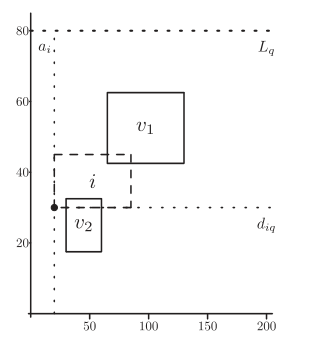
\includegraphics[width=6cm]{bap-assign.png}}
	\caption{Example of rectangle packing problem \TODO{Update Image}}
	\label{fig:packexample}
\end{figure}

%%-------------------------------------------------------------------------------
%
\section{Problem Formulation}
\label{sec:problemformulation}
The MILP is formulated with two sets of constraints: rectangle packing constraints and battery dynamics constraints. This section will progressively construct the Position Allocation MILP. A MILP is first presented purely as a rectangle packing problem that optimized over time and space. Using this MILP as a basis, new variables and battery dynamics are introduced.

\subsection{Rectangle Packing Approach}
This section presents a MILP formulation of the PAP that optimally schedules vehicles over both time and space. This section assumes that the length of the Berth ($S$), time horizon ($T$), number of incoming vehicles ($N$), charging time ($p_i$), size of the vehicle ($s_i$), and arrival time ($a_i$) for $\forall 1 \leq i \leq N$ are constant and given.

\begin{equation}\label{eq:objective}
    \sum_{i=1}^N \sum_{q=1}^Q \Big( w_i m_q + g_i \epsilon_q \Big) \\
\end{equation}

with the following constraints:

\begin{subequations}
\begin{align}
    u_i - u_j - p_j - (\sigma_{ij} - 1)T \geq 1                     \label{subeq:time}         \\
    v_i - v_j - s_j - (\delta_{ij} - 1)S \geq 1                     \label{subeq:space}        \\
    \sigma_{ij} + \sigma_{ji} + \delta_{ij} + \delta_{ji} \geq 1    \label{subeq:valid_pos}    \\
    \sigma_{ij} + \sigma_{ji} \leq 1                                \label{subeq:sigma}        \\
    \delta_{ij} + \delta_{ji} \leq 1                                \label{subeq:delta}        \\
    p_i + u_i = c_i                                                 \label{subeq:detach}       \\
    a_i \leq u_i \leq (T - p_i)                                     \label{subeq:valid_starts} \\
    c_i \leq \tau_i                                                 \label{subeq:valid_depart} \\
    \eta_i + \sum_{q=1}^Q g_{iq} r_q \leq 1                         \label{subeq:max_charge}   \\
    \eta_i + \sum_{q=1}^Q g_{iq} r_q - \lambda_i \geq 0             \label{subeq:min_charge}   \\
    \eta_i + \sum_{q=1}^Q g_{iq} r_q - \lambda_i = \eta_{\gamma_i}  \label{subeq:next_charge}  \\
    p_i \geq g_{iq}                                                 \label{subeq:gpgret}       \\
    p_i \leq g_{iq} - (1 - w_{iq})M                                 \label{subeq:gpsmol}       \\
    Mw_{iq} \geq g_{iq}                                             \label{subeq:gwgret}       \\
    0 \leq g_{iq}                                                   \label{subeq:gwsmol}       \\
    \sum_{q=1}^Q w_{iq} = 1                                         \label{subeq:wmax}
\end{align}
\end{subequations}

Where the objective function \eqref{eq:objective} is the summation over the cost of assignment of bus visit \(i\) to charger \(q\) and the usage of charger \(q\). \eqref{subeq:time} and \eqref{subeq:space} are big M constraints to ensure bus visit \(i\) is not overlapping another bus \(j\) in either time or space. \eqref{subeq:valid_pos} is similar to \eqref{subeq:time} and \eqref{subeq:space} in the sense that it verifies that the bus visit \(i\) is not overlapping bus visit \(j\) in either time or space, but it also enforces that at least one of the states must be true. \eqref{subeq:sigma} and \eqref{subeq:delta} are set in place to prevent bus visit \(i\) from being assigned to multiple positions in time or space, respectively. In other words, \eqref{subeq:time}, \eqref{subeq:space}, \eqref{subeq:valid_pos}, \eqref{subeq:sigma}, and \eqref{subeq:delta} are used together to ensure the bus visit is placed in a single valid position in both time (not encroaching on the bus in front or behind of it in the queue) and space (not allowing more than one bus to reside in the same physical space).
 Constraints \eqref{subeq:detach}, \eqref{subeq:valid_starts}, and \eqref{subeq:valid_depart} are used to enforce time constraints. \eqref{subeq:detach} states that the initial charge time plus the time on the charger is the detach time. \eqref{subeq:valid_starts} states that the arrival time is less than the initial charge time and that the initial charge time is sufficient for the bus to be on for the allotted time. \eqref{subeq:valid_depart} enforces that the detach time of bus visit \(i\) is before (or at the same as) the departure time. Constraint \eqref{subeq:wmax} is used to enforce that only a single charger may be chosen for bus visit \(i\).

\subsection{Battery Dynamics Constraints}
The set of constraints (\eqref{subeq:max_charge}, \eqref{subeq:min_charge}, and \eqref{subeq:next_charge}) are the linear battery dynamic constraints. \eqref{subeq:max_charge} does not allow bus visit \(i\) to over charge, \eqref{subeq:min_charge} does not allow the bus to be undercharged as to ensure that the bus can complete its route, and \eqref{subeq:next_charge} is the linking item that sets the initial charge for bus visit \(i\)'s next visit.

The final set of constraints(\eqref{subeq:gpgret}, \eqref{subeq:gpsmol}, \eqref{subeq:gwgret}, and \eqref{subeq:gwsmol}), are used to linearize the bilinear term \(p_i*w_{iq}\) by using big M constraints.

\subsection{Matrix Notation}\label{matrix-notation}

There are a few things to note:

\begin{itemize}
\item
  We want to convert this problem to standard LP, for our problem we
  will mainly be concerned with

  \begin{itemize}
  \item
    Inequality of \(\geq\) form
  \end{itemize}
\item
  We will be formulating the equation in the form \(Ax = b\) and
  \(Ax \geq b\) where

  \begin{itemize}
  \item
    \(A\) is a \(n \times m\) matrix
  \item
    \(x\) is a \(m \times 1\) vector
  \item
    \(b\) is a \(n \times 1\) vector
  \end{itemize}
\end{itemize}


\subsection{Position Allocation Problem}
\subsection{Charging Dynamics}

%%-------------------------------------------------------------------------------
% Example
\section{Example}

%%-------------------------------------------------------------------------------
% Conclusion
\section{Conclusion}

\subsubsection{Matrix Deconstruction}\label{matrix-deconstruction}

The constraint matrix \(A\) will be broken down into two parts:
\(A_{eq}\) for all the equality constraints and \(A_{ineq}\) for all the
inequality constraints. Both \(A_{eq}\) and \(A_{ineq}\) formulated with
two sub-matrices \(A_{pack}\) and \(A_{dynamics}\) to represent the
portion of the matrix that is utilized for the box packing constraints
and the battery dynamics constraints, respectively. For example,
\(A_{eq}\) will be represented in the following manner

\[
A_{eq} =
\begin{bmatrix}
    A_{\textrm{pack}}     \\
    A_{\textrm{dynamics}} \\
\end{bmatrix}_{eq}
\]

Where we can define the full equality as:

\[
\begin{array}{c}
    \begin{bmatrix}
        A_{\textrm{pack}}     \\
        A_{\textrm{dynamics}} \\
    \end{bmatrix}_{eq}
    \begin{bmatrix}
        x_{\textrm{pack}}     \\
        x_{\textrm{dynamics}} \\
    \end{bmatrix}_{eq} =
    \begin{bmatrix}
        b_{\textrm{pack}}     \\
        b_{\textrm{dynamics}} \\
    \end{bmatrix}_{eq} \\
    \\
    A_{eq} x_{eq} = b_{eq} \\
\end{array}
\]

Similarly for the inequality constraints:

\[
\begin{bmatrix}
    A_{\textrm{pack}}     \\
    A_{\textrm{dynamics}} \\
\end{bmatrix}_{ineq}
\begin{bmatrix}
    x_{\textrm{pack}}     \\
    x_{\textrm{dynamics}} \\
\end{bmatrix}_{ineq} \geq
\begin{bmatrix}
    b_{\textrm{pack}}     \\
    b_{\textrm{dynamics}} \\
\end{bmatrix}_{ineq}
\]

Finally, the entire constraint formulation will be written as:

\begin{subequations}
\begin{align}
    \begin{bmatrix}
        A_{\textrm{pack}}     \\
        A_{\textrm{dynamics}} \\
    \end{bmatrix}_{eq}
    \begin{bmatrix}
        x_{\textrm{pack}}     \\
        x_{\textrm{dynamics}} \\
    \end{bmatrix}_{eq} =
    \begin{bmatrix}
        b_{\textrm{pack}}     \\
        b_{\textrm{dynamics}} \\
    \end{bmatrix}_{eq} \\
    \begin{bmatrix}
        A_{\textrm{pack}}     \\
        A_{\textrm{dynamics}} \\
    \end{bmatrix}_{ineq}
    \begin{bmatrix}
        x_{\textrm{pack}}     \\
        x_{\textrm{dynamics}} \\
    \end{bmatrix}_{ineq} \geq
    \begin{bmatrix}
        b_{\textrm{pack}}     \\
        b_{\textrm{dynamics}} \\
    \end{bmatrix}_{ineq}
\end{align}
\end{subequations}

\subsection{Formulating $A_{pack}$}

\subsubsection{Formulating $A_{pack_{eq}}$}

The components that make up the equality constraints for the box packing
problem are:

\begin{itemize}
\item
  \(p_i + u_i = c_i\)
\item
  \(\sum_{q=1}^Q w_{iq} = 1\)
\end{itemize}

Placing them together in \(A_{eq}\) results in:

\begin{equation}
\begin{array}{c}
    A_{eq} =
    \begin{bmatrix}
        A_{detach_{N \times 2N}} & \vmathbb{0}_{N \times NQ} \\
        \vmathbb{0}_{N \times 2N} & A_{w_{N \times NQ}}      \\
    \end{bmatrix}_{2N \times (2N + NQ)} \\
    x_{eq} =
    \begin{bmatrix}
        p_{i_{N \times 1}} \\
        u_{i_{N \times 1}} \\
        w_{iq_{NQ \times 1}} \\
    \end{bmatrix}_{2N + NQ}
    b_{eq} =
    \begin{bmatrix}
        c_{i_{N \times 1}} \\
        \vmathbb{1}_{N \times 1} \\
    \end{bmatrix}_{2N \times 1} \\
    \\
    \begin{bmatrix}
        A_{detach_{N \times 2N}}    & \vmathbb{0}_{N \times NQ} \\
        \vmathbb{0}_{N \times 2N} & A_{w_{N \times NQ}}          \\
        \vmathbb{0}_{N \times 2N} & A_{v_{N \times NQ}}          \\
    \end{bmatrix}
    \begin{bmatrix}
        p_{i_{N \times 1}} \\
        u_{i_{N \times 1}} \\
        w_{iq_{NQ \times 1}} \\
    \end{bmatrix}
    =
    \begin{bmatrix}
        c_{i_{N \times 1}} \\
        \vmathbb{1}_{N \times 1} \\
        v_{i_{N \times 1}} \\
    \end{bmatrix}
\end{array}
\end{equation}

Where

\subsubsection{Formulating $A_{pack_{ineq}}$}
The components that make up the inequality constraints for the box
packing problem are

\begin{itemize}
\item
  \(u_j - u_i - p_i - (\sigma_{ij} - 1)T \geq 1\)
\item
  \(v_j - v_i - s_i - (\delta_{ij} - 1)S \geq 1\)
\item
  \(\sigma_{ij} + \sigma_{ji} + \delta_{ij} + \delta_{ji} \geq 1\)
\item
  \(\sigma_{ij} + \sigma_{ji} \leq 1\)
\item
  \(\delta_{ij} + \delta_{ji} \leq 1\)
\item
  \(a_i \leq c_i \leq (T - p_i)\)
\item
  \(c_i \leq \tau_i\)
\item
  \(p_i \geq g_{iq}\)
\item
  \(p_i \leq g_{iq} - (1 - w_{iq})M\)
\item
  \(Mw_{iq} \geq g_{iq}\)
\item
  \(0 \leq g_{iq}\)
\end{itemize}

\(A_{ineq}\) takes the form of:

\begin{table*}[!t]
\begin{equation}
\setlength{\arraycolsep}{2pt}
\renewcommand{\arraystretch}{0.8}
\begin{array}{c}
    A_{ineq} =
    \begin{bmatrix}
	A_{time_{\Xi \times (2\Xi + 2N)}}    & \vmathbb{0}_{\Xi \times (3\Xi + 4N + 3NQ)} & \cdots                                   & \cdots                     & \cdots                             & \cdots                           & \cdots                     & \cdots                & \cdots                    \\
	\vmathbb{0}_{\Xi \times (2\Xi + 2N)} & A_{queue_{\Xi \times (2\Xi + 2N)}}         & \vmathbb{0}_{\Xi \times (\Xi + 2N)}      & \cdots                     & \cdots                             & \cdots                           & \cdots                     & \cdots                & \cdots                    \\
	\vmathbb{0}_{N \times 2N}            & A_{\sigma_{N \times \Xi}}                  & \vmathbb{0}_{N \times (2N + 3NQ)}        & A_{\delta_{N \times \Xi}}  & \vmathbb{0}_{N \times (2\Xi + 2N)} & \cdots                           & \cdots                     & \cdots                & \cdots                    \\
	\vmathbb{0}_{N \times 2N}            & -A_{\sigma_{N \times \Xi}}                 & \vmathbb{0}_{N \times (3\Xi + 4N + 3NQ)} & \cdots                     & \cdots                             & \cdots                           & \cdots                     & \cdots                & \cdots                    \\
	\vmathbb{0}_{N \times (2\Xi + 2N)}   & \vmathbb{0}_{N \times (2N)}                & \cdots                                   & -A_{\delta_{N \times \Xi}} & \vmathbb{0}_{N \times (2N + 3NQ)}  & \cdots                           & \cdots                     & \cdots                & \cdots                    \\
	\vmathbb{0}_{N \times (4\Xi + 4N)}   & \cdots                                     & \cdots                                   & \cdots                     & -A_{a_{N \times N}}                & \vmathbb{0}_{N \times (N + 3NQ)} & \cdots                     & \cdots                & \cdots                    \\
	\vmathbb{0}_{N \times (4\Xi + 5N)}   & \cdots                                     & \cdots                                   & \cdots                     & \cdots                             & -A_{c_{N \times N}}              & \vmathbb{0}_{N \times 3NQ} & \cdots                & \cdots                    \\
	\vmathbb{0}_{N \times (4\Xi + 5N)}   & \cdots                                     & \cdots                                   & \cdots                     & \cdots                             & -A_{c_{N \times N}}              & \vmathbb{0}_{N \times 3NQ} & \cdots                & \cdots                    \\
	\vmathbb{0}_{4N \times (4\Xi + 6N)}  & \cdots                                     & \cdots                                   & \cdots                     & \cdots                             & \cdots                           & A_{gg_{4N \times NQ}}      & A_{gw_{4N \times NQ}} & \vmathbb{1}_{4N \times NQ} \\
    \end{bmatrix}_{(2\Xi + 10N) \times (4\Xi + 6N + 3NQ)}                                                                                                                                                                                                                                                                       \\
	\\
    x_{ineq} =
    \begin{bmatrix}
	u_{i_{N \times 1}} \\ p_{i_{N \times 1}} \\ \sigma_{ij_{\Xi \times 1}} \\ \vmathbb{1}_{\Xi \times 1} \\ v_{i_{N \times 1}} \\ s_{i_{N \times 1}} \\ \delta_{ij_{\Xi \times 1}} \\ \vmathbb{1}_{\Xi \times 1} \\ a_{i_{N \times 1}} \\ c_{i_{N \times 1}} \\ q_{iq_{NQ \times1}} \\w_{iq_{NQ \times 1}} \\ \vmathbb{1}_{NQ \times 1} \\
    \end{bmatrix}_{(4\Xi + 6N + 3NQ) \times 1}
    b_{ineq} =
    \begin{bmatrix}
	\vmathbb{1}_{\Xi \times 1} \\ \vmathbb{1}_{\Xi \times 1} \\ \vmathbb{1}_{N \times 1} \\ -\vmathbb{1}_{N \times 1} \\ -\vmathbb{1}_{N \times 1} \\ -c_{i_{N \times N}} \\ -(T-p_i)_{N \times N} \\ -\tau_{i_{N \times N}} \\ -p_{i_{N \times 1}} \\ p_{i_{N \times 1}} \\ \vmathbb{0}_{2N \times 1}
    \end{bmatrix}_{(5\Xi + 7N) \times 1}
\end{array}
\end{equation}\\
\end{table*}

\subsection{Formulating $A_{dynamics}$}

\subsubsection{Formulating $A_{dynamics_{eq}}$}
The components that make up the equality constraint for the dynamics problem are

\begin{itemize}
    \item
    $\eta_{\gamma_i} = \eta_i + g_{iq} r_q - \lambda_i$
\end{itemize}

$A_{dynamics}$ takes the form of:

\begin{equation}
\begin{array}{c}
	A_{eq} =
	\begin{bmatrix}
		A_{\textrm{init charge}_{N \times N}}       & \vmathbb{0}_{N \times (N+NQ)} \\
		A_{\textrm{next charge}_{N \times 2N + NQ}} & \cdots                       \\
	\end{bmatrix}_{2N \times (2N + NQ)} \\
	x_{eq} =
	\begin{bmatrix}
		\eta_{\i_{N \times 1}}   \\
		g_{iq_{NQ \times 1}}     \\
		\lambda_{i_{N \times 1}} \\
	\end{bmatrix}_{(2N + NQ) \times 1}
	b_{eq} =
	\begin{bmatrix}
		\eta_{i_{N \times 1}} \\
		\eta_{\gamma_{i}\; N \times 1} \\
	\end{bmatrix}_{2N \times 1}
\end{array}
\end{equation}

\(A_{dyanmics_{ineq}}\) takes the form of:

\begin{equation}
\begin{array}{c}
    A_{ineq} =
    \begin{bmatrix}
	-A_{\textrm{max charge}_{N \times (N+NQ)}} & \vmathbb{0}_{N \times N}        \\
	A_{\textrm{min charge}_{N \times (2N+NQ)}} & \cdots                         \\
	A_{\textrm{last charge}_{N \times N}}      & \vmathbb{0}_{N \times (N + NQ)} \\
    \end{bmatrix}_{3N \times (2N + NQ)} \\
    x_{ineq} =
    \begin{bmatrix}
	\eta_{i_{N \times 1}} \\
	g_{iq_{NQ \times 1}} \\
    \end{bmatrix}_{(2N + NQ) \times 1}
    b_{ineq} =
    \begin{bmatrix}
	-\vmathbb{1}_{N + NQ \times 1} \\
	\vmathbb{0}_{2N + NQ \times 1} \\
	H_{final}*\vmathbb{1}_{A \times 1} \\
    \end{bmatrix}_{3N \times 1}
\end{array}
\end{equation}

\subsection{Putting it back together}\label{putting-it-back-together}

\begin{equation*}
\begin{array}{c}
    \begin{bmatrix}
	A_{\textrm{pack}}     \\
	A_{\textrm{dynamics}} \\
    \end{bmatrix}_{eq}
    \begin{bmatrix}
	x_{\textrm{pack}}     \\
	x_{\textrm{dynamics}} \\
    \end{bmatrix}_{eq} =
    \begin{bmatrix}
	b_{\textrm{pack}}     \\
	b_{\textrm{dynamics}} \\
    \end{bmatrix}_{eq} \\
    \begin{bmatrix}
	A_{\textrm{pack}}     \\
	A_{\textrm{dynamics}} \\
    \end{bmatrix}_{ineq}
    \begin{bmatrix}
	x_{\textrm{pack}}     \\
	x_{\textrm{dynamics}} \\
    \end{bmatrix}_{ineq} \geq
    \begin{bmatrix}
	b_{\textrm{pack}}     \\
	b_{\textrm{dynamics}} \\
    \end{bmatrix}_{ineq}
\end{array}
\end{equation*}

May also be represented as

\scriptsize

\begin{equation}
\begin{array}{c}
A_{eq} =
\begin{bmatrix}
    \begin{Bmatrix}
	A_{detach_{N \times 2N}}    & \vmathbb{0}_{N \times NQ} \\
	\vmathbb{0}_{N \times 2N} & A_{w_{N \times NQ}}          \\
	\vmathbb{0}_{N \times 2N} & A_{v_{N \times NQ}}          \\
    \end{Bmatrix}_{3N \times (2N + NQ)}
    \begin{Bmatrix}
	\vmathbb{0}
    \end{Bmatrix}_{3N \times (2N + NQ)} \\
    \begin{Bmatrix}
	\vmathbb{0}_{}
    \end{Bmatrix}_{NA \times (2N + NQ)}
    \begin{Bmatrix}
	A_{\textrm{next charge}_{N \times 2N + NQ}}
    \end{Bmatrix}_{NA \times (2N + NQ + A)} \\
\end{bmatrix}_{(3N + NA) \times (4N + NQ + A)} \\
x_{eq} =
\begin{bmatrix}
    \begin{Bmatrix}
	p_{i_{N \times 1}} \\
	u_{i_{N \times 1}} \\
	w_{iq_{NQ \times 1}} \\
    \end{Bmatrix}_{2N + NQ} \\
    \begin{Bmatrix}
	\eta_{\Gamma_{i\; N \times 1}} \\
	g_{iq_{NQ \times 1}}           \\
	\lambda_{i_{N \times 1}}       \\
    \end{Bmatrix}_{(2N + NQ + A) \times 1}
\end{bmatrix}_{(4N + 2NQ + A) \times 1}
b_{eq} =
\begin{bmatrix}
    \begin{Bmatrix}
	c_{i_{N \times 1}} \\
	\vmathbb{1}_{N \times 1} \\
	v_{i_{N \times 1}} \\
    \end{Bmatrix}_{3N \times 1} \\
    \begin{Bmatrix}
	\eta_{\gamma_{i}\; N \times 1} \\
    \end{Bmatrix}_{N \times 1}
\end{bmatrix}_{4N \times 1} \\
\begin{bmatrix}
    \begin{Bmatrix}
	A_{detach_{N \times 2N}}    & \vmathbb{0}_{N \times NQ} \\
	\vmathbb{0}_{N \times 2N} & A_{w_{N \times NQ}}          \\
	\vmathbb{0}_{N \times 2N} & A_{v_{N \times NQ}}          \\
    \end{Bmatrix}_{3N \times (2N + NQ)}
    \begin{Bmatrix}
	\vmathbb{0}
    \end{Bmatrix}_{3N \times (2N + NQ)} \\
    \begin{Bmatrix}
	\vmathbb{0}_{}
    \end{Bmatrix}_{NA \times (2N + NQ)}
    \begin{Bmatrix}
	A_{\textrm{next charge}_{N \times 2N + NQ}}
    \end{Bmatrix}_{NA \times (2N + NQ + A)} \\
\end{bmatrix}
\begin{bmatrix}
    \begin{Bmatrix}
	p_{i_{N \times 1}} \\
	u_{i_{N \times 1}} \\
	w_{iq_{NQ \times 1}} \\
    \end{Bmatrix}_{2N + NQ} \\
    \begin{Bmatrix}
	\eta_{\Gamma_{i\; N \times 1}} \\
	g_{iq_{NQ \times 1}}           \\
	\lambda_{i_{N \times 1}}       \\
    \end{Bmatrix}_{(2N + NQ + A) \times 1}
\end{bmatrix} \\
=
\begin{bmatrix}
    \begin{Bmatrix}
	c_{i_{N \times 1}} \\
	\vmathbb{1}_{N \times 1} \\
	v_{i_{N \times 1}} \\
    \end{Bmatrix}_{3N \times 1} \\
    \begin{Bmatrix}
	\eta_{\gamma_{i}\; N \times 1} \\
    \end{Bmatrix}
\end{bmatrix}_{4N \times 1}
\end{array}
\end{equation}

%%================================================================================
% Bibliography
\bibliographystyle{IEEEtran}
\bibliography{main}

%%%%%%%%%%%%%%%%%%%%%%%%%%%%%%%%%%%%%%%%%%%%%%%%%%%%%%%%%%%%%%%%%%%%%%%%%%%%%%%%%
\end{document}
